\chapter{Introduction}
\label{chapter:introduction}

Nowadays companies have to be increasingly flexible due to a fast changing market in order to remain
competitive. Hence, business processes have to be highly adaptable and extensible to the current
market requirements. Furthermore, most business processes within modern companies rely on various
different software products which therefore have to be easily adaptable as well. This statement is
emphasised by \cite{flexible_software}:

\msQuote{Most executives say that their businesses are changing faster than their IT organizations
can keep critical systems current. Yet IT cannot afford to make any major modifications because so
much of the technology budget is devoted to incremental maintenance.}

To base a software product on a service oriented architecture constitutes one possibility to support
the flexibility and adaptability requirements. Furthermore, this architecture can be provided with an
interface, which enables the dynamic combination and orchestration of services without any
programming skills, similar to ``Mashup Composers''. These mashup composers provide mechanisms to
combine the ever growing number of data sources exhibited by the world wide web as well as local resources like
databases and Excel spreadsheets. Integrating open APIs and combining, filtering or merging these
sources can produce results which were not originally provided by either source and therewith make
the data more valuable.

Hence, this thesis deals with the evaluation of three mashup composers, which enable the fast and
easy integration of multiple data sources within a mashup. The analysis of the evaluation result
finally reveals promising approaches and some major problems, which are not handled by the tools
yet. After having identified these problems a solution can be elaborated which leads to the
implementation of the Component Framework.

Therefore, the long-term objective for providing an interface, which can be used by end-users to
adapt existing applications to changing business processes or to create new applications for new
requirements, should be the enhancement of mashup composers from simple data aggregation and display
tools, to composers for complex and business capable applications.

The following section introduces the business scenario which led to the idea of implementing the
basis framework for such a composer and hence can be seen as an adequate use case for the Component
Framework.

\section{Problem Statement and Motivation}
\label{sec:scenario}

The following scenario introduces a common problem of business processes within companies. Many
different users with different roles are working on a single process, but require different software
products or slightly adapted versions of such a product. Hence, an appropriate software solution
should be highly adaptable for various different roles and situations.

\subsection{A Case Study}

Let's assume an air ambulance company which has to process multiple flights a day with all the
common steps that have to be taken, the events that can occur and the different roles that are involved.

\subsubsection{An Air Ambulance Process}

First of all an insurance company commissions the air ambulance company to transport a patient from
destination A to destination B. As next step the air ambulance sets up a flight instruction, which
contains information about start and destination airport, the responsible hospitals, the diagnosis as
well as various personal data of the patient. Furthermore, it includes information about the flight
as well as the medical crew, which includes doctors and nurses and the flight schedule, which
provides details about the exact flight times and the necessary stopovers to either pick up another
patient or to refuel.

The following steps have to be taken before the liftoff, to guarantee a smooth transportation of the
patient from destination A to destination B.

\begin{itemize}
  \item Check the availability of an airplane. The flying hours have to be taken into account,
  because after a certain number of flying hours the airplane has to be maintained.
  \item Check the availability of all crew members. Again the flying hours have to be taken into
  account. After a certain number of flying hours each pilot has to have a regeneration phase.
  \item Organize ambulances which transport the patient to the respective airport and pick him up
  at the destination airport.
  \item Inform the so-called ``Handling'', which is responsible for acquiring several permissions at
  the intermediate and destination airports. This includes permissions for the ambulances to drive
  across the airport and pick up the patient directly at the airplane, for the tank truck to drive
  across the airport and refuel the airplane and land- and overflight-permissions.
  \item Send preflight information to the concerning airports. This information includes details
  about the airplane itself, a unique flight number, the schedule and the pilots personal data.
  \item Organize a hotel for the crew, in case its members have to stay overnight.
  \item Check airports for business hours and customs and send passport information of the crew to
  the airport which controls the respective passports.
  \item Organize the catering of the crew and passengers.
  \item On the basis of the schedule the dispatcher generates one or more flight plans
  dependent on the number of stopovers.
  \item Finally, the crew has to be informed about the schedule.
\end{itemize}

Having completed all of these steps the airplane can lift off. During the whole flight, pilot and
dispatcher or the organization center respectively are in contact and communicate to prevent or
deal with occurring problems:

\begin{itemize}
  \item Shortening or lengthening of the flight time due to the wind situation. Therefore,
  ambulances at the destination airports have to be informed. Furthermore, headwind leads to a
  higher fuel consumption and hence can lead to the necessity of an additional intermediate stop to
  refuel.
  \item Foul weather can cause the close-down of the destination airport. Hence, an alternative has
  to be organized.
  \item The destinations' hospital, which was organized by the commissioning insurance company,
  cannot assure the necessary medical care. Hence, an alternative hospital has to be organized.
  \item The airplane itself can have a technical problem. Therefore, the air traffic administration
  has to be informed, which tries to solve the problem during the flight and initiates an emergency
  landing if necessary.
\end{itemize}

Finally, if all events were handled successfully and the patient has arrived at the predefined
destination, the case can be closed.

The described air ambulance company includes various different jobs and roles respectively.

\subsubsection{The Involved Roles}

The \textbf{head of the company} mainly wants to monitor the actual incidents. Therefore, a suitable
software product should provide means to monitor various cases or flights simultaneously. In more
detail this means that one part of the user interface has to display one or more flights in its
planning phase, indicating the processed and still open steps and the other part should display
flights which are in execution phase. Therefore, this part includes information about the current location of the
airplane, the actual delay, the crew, the patient and many more things as desired.

\textbf{Employees of the organization center} do not only need to monitor the current operations
but also need a software product which supports them in their organizational work. Therefore, a
user interface for entering flights, setting up the preflight information, informing ambulances and
much more is required.\newline
That means that the final software product for such an employee should include the same or if
necessary an adapted version of the user interface the head of the company uses, as well as a user
interface which perfectly supports the planning phase of a flight. Furthermore, the monitoring
component should be able to dispatch events as soon as one of the described problems occurs. Hence,
the organizational staff can be informed automatically and the necessary reactions can be initiated.

The \textbf{dispatcher} finally needs a software product which integrates a user interface for
creating flight plans and a more sophisticated monitoring tool which fetches more technical
information about the airplane and displays the route and the exact position of the airplane on a
map. As the dispatcher has to supervise multiple flights in parallel the software product should
again provide an interface to display multiple flights on the same site or at least provide the
functionality to switch between them easily. Furthermore, it should integrate a simple method to
communicate with each of the airplanes and pilots respectively.

To sum up, each of these roles requires a software product which reuses components of another role
and extends it with some role specific parts and features respectively. That means that each role
specific application can be seen as an aggregation of multiple components.

\subsubsection{Conclusion}

This requirement led to the idea of implementing a framework which provides a catalog of simple base
components which can be assembled and connected with a few mouse clicks and finally constitute a
full-fledged application.\newline An extensive search on the Internet revealed similar approaches
(e.g., \cite{fast}, \cite{riena}, \cite{swordfish_whitepaper}, \cite{websphere_dashboard}.
\cite{aris_dashboard}). The most promising one was the approach of mashup composer tools,
which provide a user interface for accessing and connecting various data sources and displaying the
result on a map, a simple table or every other imaginable kind of display. Each of these mashups
consists of multiple base components and thus implements the addressed architectural approach.

In order to do not invent the wheel twice, an evaluation of the most important mashup composer
tools is conducted in Chapter \ref{chapter:evaluation}, before the addressed framework is
implemented.

The following section therefore introduces some background information about mashups.  

\section{Background}

This section introduces terms which provide the necessary background
information that is needed to understand the following sections more easily.

\subsection{Mashup}
\label{sec:mashup}
As the first part of this thesis deals with mashups and mashup composer tools in the context of web
development, it is important to clarify the term mashup.

\subsubsection{Definition of a Mashup}
A mashup is a web application that combines data from two or more sources,
converts, manipulates or processes the data to make it more valuable, and
displays the output.

John Crupi and Chris Warner define mashups as follows \cite{mashup_definition}:

\msQuote{A mashup is a user-centric micro-combination of standards-based internal
and external data sources.}

\par This definition points to several characteristics of mashups \cite{mashup_definition}.

\begin{itemize}
	\item \textbf{User-centric} means that the data sources are most generally user
	consumable and that the mashups are created, utilized and interpreted by users without any
	in-depth programming skills.
	\item \textbf{Micro-Combination} stands for the combination of rather small
	data sources with small amounts of knowledge-oriented information, which can
	be much more valuable as soon as the information of the various sources is
	combined.
	\item With \textbf{Standards-based Internal and External Data}, like WSDL, REST or RSS the
	data sources do not require too much manipulation for the user to make sense of it. Typical data sources
	for mashups are public third party interfaces or APIs, like the one of Google Maps
	\cite{google_maps}, web feeds, which are provided by nearly every website that consistently
	provides new information, and in the meantime also databases, Excel-sheets, CSV-files and many
	more.
\end{itemize}

An example for a simple mashup is the use of cartographic data
in combination with location data of customers, like addresses or zip-codes. The
output of such a mashup would be, for example, Google Maps displaying the names
of the customers at their specific addresses.

The \textbf{structure} of mashups typically consists of the following three parts:
\begin{itemize}
	\item Two or more \textbf{data sources} that provide the content for the
	mashup.
	\item Some kind of \textbf{logic that enables the composition of these data sources}. This can
	range from simple operations like combining data, filtering data, adding static information to
	the data, to more sophisticated operations, like contacting a web service that manipulates the
	data in a special way.
	\item As the third and last part there has to be a possibility to \textbf{display the
	data} in a suitable way. Data can, for example, be displayed within Google Maps, in a table
	listing the data elements row by row or in some other adequate form.
\end{itemize}

\subsubsection{Types of Mashups}

Mashups can be distinguished by their target group which is either the common end-user or an
enterprise. Volker Hoyer and Marco Fischer define these two types as follows
\cite{types_of_mashups}:

\begin{itemize}
  \item \textbf{Consumer Mashups}\newline A consumer Mashup tool is mainly aimed at individuals to
  easily create Mashups for private use, e.g. personalized browser page. The Consumer Mashup is
  perhaps the best know type of Mashups. Consumer Mashups combine data elements from multiple
  sources, hiding this behind a simple unified graphical interface. Instead of opening several Web
  pages to view, for example, the weather forecast, the news and your private emails, the consumer
  is able to create an individual start page pulling the information from different sources.
  \item \textbf{Enterprise Mashups}\newline Enterprise Mashups combine existing resources, be it
  content, data or application functionality, from more than one source in enterprise environments. In contrast to
  Consumer Mashups, enterprise environments implicate additional requirements like security, quality
  or availability. In addition, Enterprise Mashups focus on integrating existing back-end systems.
  So, Enterprise Mashups have enormous potential to allow more rapid and much less expensive
  development of applications by emphasizing assembly over development, economies of scale by
  enabling high levels of reuse, and the consequent ability to rapidly get software solutions with
  the right data in the right place at the right time.
\end{itemize}

\subsection{SOA - Service Oriented Architecture}
\label{sec:service_oriented_architecture}
As we talk about connecting data sources, functions that filter, merge or combine data and web
technology and web services respectively, we have to introduce the term ``Service Oriented
Architecture''.

A service oriented architecture consists of \textbf{service providers} and \textbf{service
consumers} which are loosely coupled and exchange data via standardized communication protocols
(see Figure \ref{fig:soa}). Furthermore, services can be provided by heterogeneous systems, used
within multiple domains and do not rely on their implementation platform or language
\cite{nicolai}. In order to enable the interoperability of all these services, each of them has to
provide a well defined interface, which is commonly described with an XML-based description
language.

\begin{figure}
	\centering
		\fbox{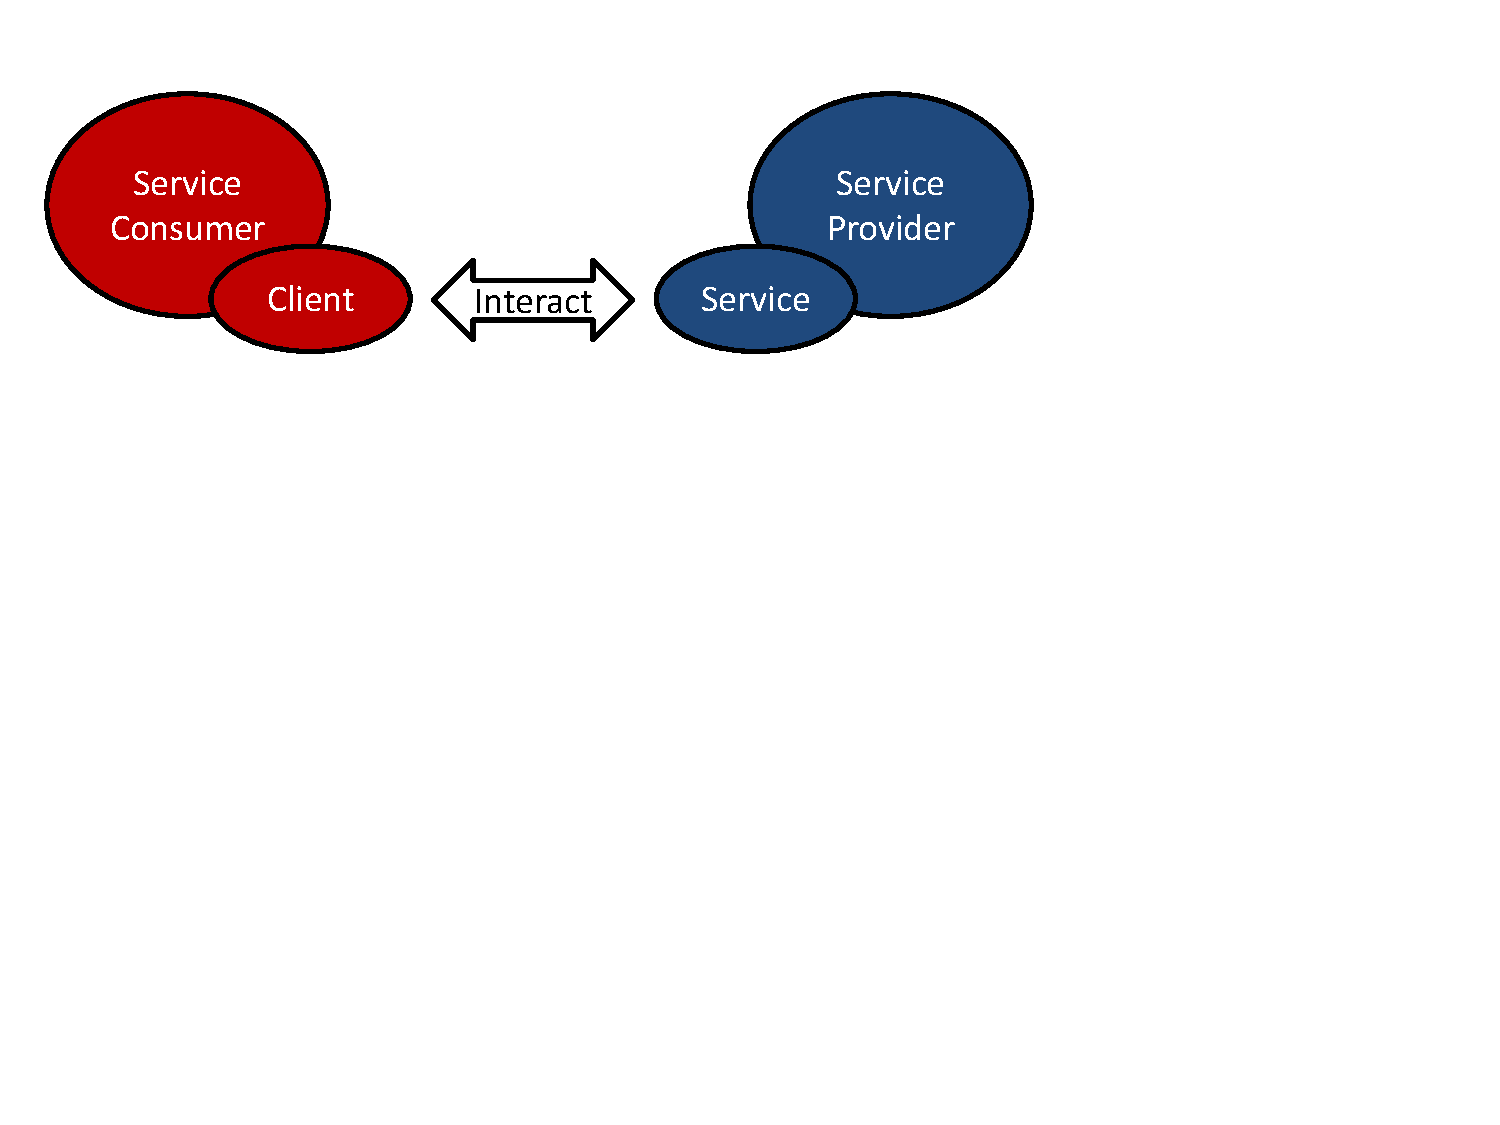
\includegraphics[width=0.8\textwidth]{Bilder/soa.pdf}}
	\caption{Service Oriented Architecture}
	\label{fig:soa}
\end{figure}

A very important design principle with respect to mashups and mashup composer tools is the ``Service
Composability'' principle, which encourages the design of services in a loosely coupled manner and
hence can be reused in multiple solutions that are themselves made up of composed services \cite{soa}.

\section{Related Work}

The approach, which is discussed in this thesis, is not the only one, which can be applied to
realize the discussed scenario (see Section \ref{sec:scenario}). Hence, the most interesting
approaches with respect to this thesis will be summarized subsequently.

\subsection{A Service-Oriented Approach to Document-Centric Situational Collaboration Processes}
This paper \cite{schuster2009} introduces a service-oriented approach to integrate enterprise
documents within SOA landscapes. Therefore, it represents documents as compositions of stateless
software services, which can be described, published, discovered, selected and accessed - with
respect to the SOA paradigm. Furthermore, these services can communicate based on an event-based
communication model and interact according to specified document interaction patterns.\newline The
composition of the available document services, like content, transformation, composition or layout
services, finally takes place in a mashup infrastructure, like the ones that are provided by IBM
Mashup Center, Microsoft Popfly or Yahoo Pipes.

\subsection{FAST}
The main objective of the \textit{``FAST (Fast and Advanced Storyboard Tools)''} project \cite{fast}
is to create a new visual programming environment that facilitates the development of complex
front-end gadgets, involving execution of relatively complex business processes that rely on back-end
semantic web services.\newline Instead of first building programs that orchestrate available
semantic web services and then trying to figure out how to implement interaction with the users at
given points of the process execution flow, programmers will start from the front-end gadgets that the user will see
and interact with, and then visually establish connections to back-end Web Services, going through
process execution flows if necessary.\newline
The goal of the project is to develop ``mashup-able'' gadgets that rely on semantic web services
independent of the mashup platform, which is used to display or further process the gadgets. That
means that the resulting gadgets should be deployable within all three of the inspected mashup tools or
platforms as they are called with respect to FAST. However, at the moment FAST only supports a
single target mashup platform, namely EzWeb \cite{ezweb}, which is still in beta state
\cite{fast_paper}.

\subsection{MarcoFlow}
MarcoFlow aims at going one step beyond state-of-the-art workflow management and service composition
and proposes an original model, language and running system for the composition of distributed UIs,
an approach that allows to easily bring together UIs, web services and people in a single
orchestration logic and tool. The type of applications that can be developed with MarcoFlow are
called ``distributed UI orchestrations'' \cite{marcoflow}.

However, MarcoFlow is more targeted at designing the workflow and orchestrating distributed web
services and UIs within an application which requires technical skills and a deep insight in the
workflow and the involved services. Whereas the goal of the mashup composers, like Microsoft Popfly,
Yahoo Pipes and IBM Mashup Center, and this thesis is the simple composition and adaptation of
applications on a user interface which can be handled by end-users without technical insight.

\subsection{Approaches based on the OSGi Framework}
The following two approaches extend the OSGi Framework with useful and interesting functionalities
to build a custom enterprise service bus or a multi-tier enterprise client/server application and
hence could have been used as basis for the Component Framework. However, none of the approaches is
dedicated towards visually designing applications and minimizing the required programming skills
and hence the most lightweight framework was chosen as basis.

\subsubsection{Swordfish}
Swordfish \cite{swordfish} provides an open source framework that allows application developers and
system integrators to build their own enterprise service bus (ESB), which enables the combination of
services in an easy and flexible manner. It is based on proven technologies like Apache ServiceMix
and hence on OSGi as well as on the JBI standard for messaging abstraction and message routing
between components.\newline Furthermore, the integrated Service Registry allows a loose coupling
between service providers and service consumers, which are connected dynamically at runtime. The
communication takes place directly between two services or components respectively and therefore
needs no intermediary which could become a performance bottleneck \cite{swordfish_whitepaper}.

\subsubsection{Riena}
The Riena platform \cite{riena} is a framework for building multi-tier enterprise
client/\newline server applications and therefore broadens the usage of the service oriented
architecture of OSGi by providing access to local and remote services in a transparent way.\newline Using the provided
concepts and programming model the enterprise application can be developed regardless of the target
location and the individual components can be either placed on the client or server side of
the application depending on the business requirements \cite{eclipse_riena}.\newline Furthermore,
Riena provides a redesign for the Eclipse RCP workbench which tries to simplify the navigation
within the created applications.

\subsection{Dashboards}
Related to this thesis are also dashboard applications. Stephen Fex defines a dashboard as follows
\cite{stephen_few}:

\msQuote{A dashboard is a visual display of the most important information needed to achieve one or
more objectives; consolidated and arranged on a single screen so the information can be monitored
at a glance.}

Hence, a dashboard is a software product aimed to integrate information from multiple components into
a unified display. For example, it might obtain information from the local operating system, from
applications that may be running, and from remote sites on the Web and present it as though it all
came from the same source.\newline As sophisticated dashboards can connect to nearly any data source
and are highly customizable, they are also used within enterprises to provide a dynamic read-out of
personalized, business-critical information.\newline Popular examples for dashboards which can be
used within business are the ``WebSphere Dashboard Framework''
\cite{websphere_dashboard} from IBM and the ``ARIS Performance Dashboard'' \cite{aris_dashboard}
from IDS Scheer.

Nevertheless, dashboards are not designed to let the simple information displays or widgets
communicate, exchange information or react to user inputs and hence are not applicable for the
described scenario (see Section \ref{sec:scenario}).

\subsection{Portals and Portlets}
Portals and Portlets provide a first approach to component-based UI development \cite{portlets}.
Portlets are full-fledged, pluggable Web application components which generate document markup
fragments (e.g., HTML) and can be arranged on a portal page. A portal server therefore allows users
to manage and customize such portal pages and furthermore provides single sign-on and role-based
personalization.

However, portals and portlets exhibit the same drawbacks as dashboards and hence are not applicable
as well.

\section{Research Objectives}
\label{sec:research_objectives}

Goal of this thesis is to investigate existing mashup composer tools, which are aimed at end-users
without any programming skills and provide a simple user interface for accessing and aggregating
different data sources and hence developing mashups and applications respectively. The conducted
evaluation of these tools and the adopted set of evaluation criteria should help identifying the
major lacks and missing functionality, which are required to realize a scenario like the one
introduced in Section \ref{sec:scenario}.

Hence, the major research objective is, besides the evaluation, the development of the
``Component Framework'' which tries to support the requirements of the introduced scenario. The
framework should be built on technologies which are standardized and well approved in practice,
since the target applications, which should be applicable in business as well, should be as stable,
fail-safe and secure as possible.

\section{Research Method}

As addressed in Section \ref{sec:research_objectives} the adopted research method is the evaluation
of existing mashup composer tools. Therefore, specific evaluation criteria which represent the
requirements for these tools to realize a scenario, like the one that is described in Section
\ref{sec:scenario}, are introduced, the evaluation is conducted and the final results are presented
and analyzed.

Having identified the problems which are discovered during the evaluation process and are not
solved by the existing tools, requirements for the implementation of a solution are derived.
These requirements form the basis for the prototype framework which tries to compensate the observed
limitations and is implemented as part of this thesis. Finally, to validate the feasibility of the
proposed framework a test application based on the air ambulance scenario has been developed.

\section{Structure of the Thesis}
The remainder of this thesis is structured as follows:

\textbf{Chapter \ref{chapter:evaluation}} evaluates three software products which are used to create and
design mashups. Each of them is targeted at the easy access and aggregation of data in order to
produce output that is more valuable than the separate data input streams.

\textbf{Chapter \ref{chapter:requirements}} discusses the evaluation results and formulates a set of
requirements for a software product which eliminates the weaknesses of the evaluated products and
provides means for realizing the scenario introduced in Section \ref{sec:scenario}.

\textbf{Chapter \ref{chapter:osgi}} introduces and illustrates the well-known OSGi Framework, which
provides the basis for the developed prototype framework, which is called ``Component Framework''. The
Component Framework is especially implemented for this master thesis and tries to support the
introduced requirements.

\textbf{Chapter \ref{chapter:applications}} introduces two applications which are based on the implemented
framework and therefore demonstrate the feasibility of the underlying concepts.

\textbf{Chapter \ref{chapter:summary}} concludes the thesis with a summary.